\documentclass[10pt,twocolumn,letterpaper]{article}

%------------------------------------------------------------------------------
% Packages
%------------------------------------------------------------------------------
\usepackage{iccv}
\usepackage{times}
\usepackage{epsfig}
\usepackage{graphicx}
\usepackage{amsmath}
\usepackage{amssymb}
% Include other packages before hyperref.
\usepackage[breaklinks=true,bookmarks=false]{hyperref}

%------------------------------------------------------------------------------
% Preamble
%------------------------------------------------------------------------------

% *** Uncomment this line for the final submission
\iccvfinalcopy 

% Paper ID.
\def\iccvPaperID{****} % *** Enter the ICCV Paper ID here
\def\httilde{\mbox{\tt\raisebox{-.5ex}{\symbol{126}}}}

% Pages are numbered in submission mode, and unnumbered in camera-ready
%\ificcvfinal\pagestyle{empty}\fi
\setcounter{page}{1}

\newcommand{\I}{\mathcal{I}}
\newcommand{\D}{\mathcal{D}}

%------------------------------------------------------------------------------
% Document
%------------------------------------------------------------------------------

\begin{document}

\title{
  Autonomous Population Estimation in an Explorable Environment using a Counting
  CNN and Reinforcement Learning
}

\author{
  A. G. Musco, M. Hoai\\
  Stony Brook University\\
  Stony Brook, NY\\
  {\tt\small amusco@cs.stonybrook.edu, minhhoai@cs.stonybrook.edu}
}

\maketitle

%------------------------------------------------------------------------------
% Abstract
%------------------------------------------------------------------------------

\begin{abstract}
  Estimating the population size of some identifiable target in an explorable
  environment has many real-world applications, including animal population
  surveys, disaster relief operations, and crowd control at sporting events. In
  this paper, we describe a method to train an autonomous drone to count
  members of a target population in an explorable enviroment using a Counting
  CNN and reinforcement learning though OpenAI Gym and Gazebo.
\end{abstract}

%------------------------------------------------------------------------------
% SECTION 0: Introduction
%------------------------------------------------------------------------------

\section{Introduction}

\subsection{Motivation}

  In many applications where a target population must be estimated in an open
  environment, it is desireable to have an autonomous agent intelligently
  explore without direct operator feedback. Such intelligent behavior could
  allow for a single operator to supervise a fleet of autonomous agents without
  the need to directly control any agent individually, which could lead to
  dramatic boosts in efficiency and decreased assesment time.

\subsection{Methodology}

  The work described in this paper is split into two parts: 1) training a CNN
  to count the targets in the current frame, and 2) using this trained CNN to
  maximize the targets observed by a drone in a simulated environment. 
  
  For part 1, we used O\~noro and L\'opez-Sastre's \textit{counting CNN} model
  \cite{onoro2016} to train a CNN to output an accurate \textit{density map}
  from an input image and it's corresponding \textit{dot image}. Instead of
  manually labelling training images, we utilize Gazebo to simulate a virtual
  environment in order to generate input images and their corresponding dot
  images automatically.

  For part 2, we used the trained CNN to count targets viewed by a simulated
  drone within Gazebo in a reinforcment learning context. In each episode, the
  drone takes actions in order to maximize the count of targets in the current
  frame. This reward-seeking behavior allows an agent to automatically assess
  an environment for a target population without direct operator control.

  It is worth mentioning that several components of this experiment make use of
  \textit{Gazebo}, a simulation environment used to develop and test robotic
  components. The code associated with this paper includes several Gazebo
  plugins used to generate training data, as well as to provide the environment
  used for reinforcement learning.

%------------------------------------------------------------------------------
% SECTION 1: Counting CNN
%------------------------------------------------------------------------------

\section{Counting CNN}

  The Counting CNN is based off the work by O\~noro and L\'opez-Sastre in
  \cite{onoro2016}. Using the architecture desribed in this paper, we
  implemented a 6-layer CNN to learn a mapping from $64 \times 64 \times 3$
  color images to $16 \times 16 \times 1$ density maps using the
  \textit{TensorFlow} Python library. Once the density map for a particular
  image has been predicted, the in-frame population count can be calculated by
  integrating the raw pixel values over the entire density map.

  More formally, let $C(\I)$ denote the true count of the target population
  within the image $\I \in \mathbb{R}^{64 \times 64 \times 3}$. Suppose there
  exists a function $f: \mathbb{R}^{64 \times 64 \times 3} \rightarrow
  \mathbb{R}^{16 \times 16 \times 1}$ such that each pixel in the resulting
  density map $f(\I)$ encodes the target population ``mass'' in the
  corresponding pooled $4 \times 4$ pixel region of the input image, and that
  the sum of all such pixels is equal to $C(\I)$:
  \begin{align}
    C(\I) = \sum_{p \in f(\I)} {f(\I)}_p
  \end{align}

  \begin{figure*}
  \begin{center}
  \fbox{
    %\rule{0pt}{2in} 
    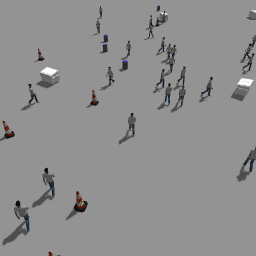
\includegraphics[width=0.3\linewidth]{img/training-img.png} \quad
    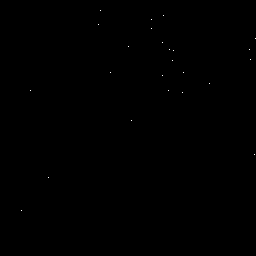
\includegraphics[width=0.3\linewidth]{img/training-img-dots.png} \quad
    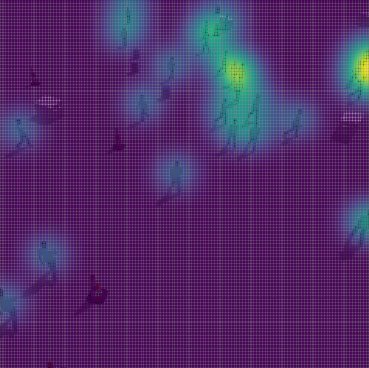
\includegraphics[width=0.3\linewidth]{img/training-img-dens.png} 
    %\rule{.9\linewidth}{0pt}
  }
  \end{center}
     \caption{Image generated from Gazebo with its corresponding dot image and
     density map ($\sigma^2 = 10$)}
  \label{fig:trainimg}
  \end{figure*}

  We thus define the following surrogate objective to counting the target
  population: learning the function $f$ mapping $\I$ to $\D$. Once an estimate
  $f^*$ has been learned, we can count the target population in a new image
  $\I'$ by producing $f^*(\I')$ and summing over the resulting map:
  \begin{align}
    C(\I') = \sum_{p \in f(\I')} {f(\I')}_p \approx \sum_{p \in f^*(\I')}
      {f^*(\I')}_p
  \end{align}

  This converts population counting into a regression problem which can be
  trained using a Convolutional Neural Network. To generate the density maps to
  train on, we first generate a binary dot image the same shape as the input
  image with a single ``hot'' pixel at the coordinates of each target class
  member in the frame. We then apply a Gaussian filter to distribute the
  ``mass'' more evenly throughout the image, which transforms the problem from
  binary detection into continuous regression. Note the important property that
  applying a Gaussian filter doesn't alter the total intensity- thus the
  sum of all pixels before applying the filter should be approximately equal to
  the sum after applying the filter. \footnote{There are cases, such as along
  the image boundary, where the Gaussian ``blob'' may be truncated, resulting
  in a loss of mass. This loss is assumed to be small, however, and within
  acceptable bounds to be considered random noise.}

%------------------------------------------------------------------------------

\subsection{Training}


  In the original paper by O\~noro and L\'opez-Sastre, the Counting CNN was
  trained on images that were manually annotated with a single dot for each
  member of the target class. This proves to be a time consuming and laborious
  task, which limits the amount of training data usable by the Counting CNN.

  Instead of manually labelling real-world images, we leveraged Gazebo's
  virtual environment in order to automatically generate training images and
  their corresponding dot image labels. This provides a simple way to generate
  data on-demand for \textit{any} desired population class, without the need to
  manually annotate each image. The only requirement is a sufficiently detailed
  model of the target class in the form of a mesh and a texture which can be
  fed into the Gazebo virtual environment. 

  Figure~\ref{fig:trainimg} displays a typical training image along with its
  dot image. In this example a simple pedestrian is the target class to be
  counted, though the environment includes several other objects such as
  traffic cones and dumpsters in order to provide some noise and prevent
  over-fitting. The figure also includes an example density map overlayed on
  top of the source image, which represets the approximate ``mass-per-pixel''
  of the target class. This density map is generated from the dot image by
  convolving with a Gaussian filter with zero mean and a tunable variance
  $\sigma^2$.

%------------------------------------------------------------------------------

\subsection{CNN Architecture}

  As mentioned above, the Counting CNN trained in this experiment consisted of
  6 primary convolutional layers with 2 pooling layers after the first and
  second convolutions. The convolutional layers gradually expand the output to
  1,000 feature maps, while simultaneously reducing the patch size from $64
  \times 64$ to $16 \times 16$. This provides the network enough flexibility to
  learn intricate representations of the target class, as well as
  representations of common non-class signals\footnote{ e.g.\ objects that
  commonly appear in input images but are not countable as members of the
  target class.} to be ignored. The last two layers of the network collapse the
  feature maps into a single output channel. This output channel is the learned
  density map with which an estimated population count can be produced.

  Batch normalization~\cite{ioffeS15} was applied after each covolutional layer
  in order to reduce covariate shift. This was observed to occur due to the
  varying scales of input images\footnote{Images from higher altitudes
  had a much different intensity distribution that images much closer to the
  scene, and resulted in vanishing gradients in the lower convolutional
  layers.}.

%------------------------------------------------------------------------------

\subsection{Data Pipeline}

  Rather than passing large raw images through the Counting CNN, the network
  takes as input patches of size $64 \times 64 \times 3$, and produces an
  output density map of size $16 \times 16 \times 1$. This provides a more
  consistent and reliable prediction model, where images of any size can be
  broken up into a dense grid of patches that are predicted individually, then
  reconstructed into a composite prediction for the entire image.

%------------------------------------------------------------------------------

\subsection{Results}
  \begin{figure}
  \begin{center}
  \fbox{
    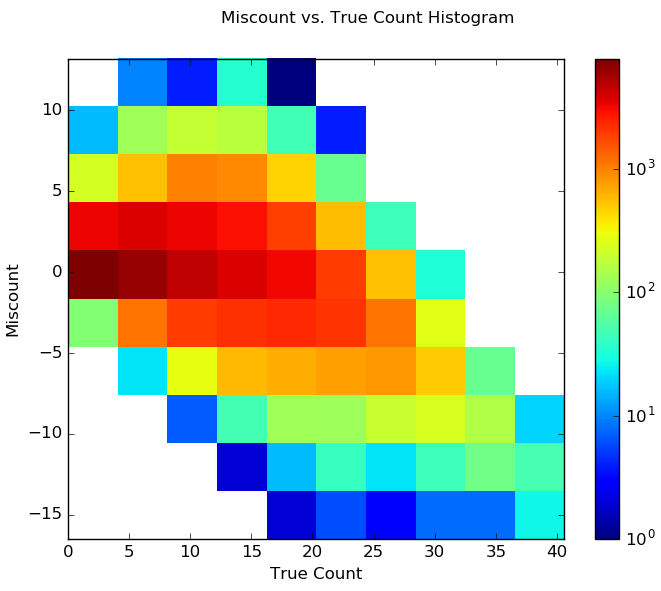
\includegraphics[width=0.9\linewidth]{img/hist.png} \quad
  }
  \end{center}
     \caption{Histogram of miscount errors with respect to total in-frame
     population count (\textit{i.e.\ scale of the image})}
  \label{fig:hist}
  \end{figure}

  As is shown in Figure \ref{fig:hist}, the Counting CNN performed well for
  images with only a few pedestrians in-frame. As the number of pedestrians
  in-frame grows, there is a trend for the CNN to undercount (\textit{this can
  also be seen in the bottom row of Figure \ref{fig:ex1}}). We attribute this
  to the fact that the Counting CNN adapts to counting at a particular scale,
  and images at low angles tend to include pedestrians at a spectrum of scales.
  In other words, the Counting CNN is not capable of assigning a far pedestrian
  with the same weight as a near pedestrian, and therefore undercounts
  pedestrians in the background. This issue can be remedied by training
  multiple Counting CNNs at differing scales, and then combining the output of
  these networks in a fully-connected layer. This is implemented in the
  \textit{Hydra CCNN} in \cite{onoro2016}, but was not implemented here to keep
  the network simple and fast.

  Figure \ref{fig:ex1} showcases some sample prediction density maps along with
  their total predictions. As is implied in Figure \ref{fig:hist}, the Counting
  CNN performs well for images with less than 30 pedestrians at similar scale,
  but begins to undercount for pictures with many pedestrians varying scales.
  Note that in the samples provided the Counting CNN has learned to ignore many
  of the non-class signals (\textit{traffic cones, barrels, dumpsters}) as well
  as account for mild occlusion of pedestrians.

  \begin{figure*}
  \begin{center}
  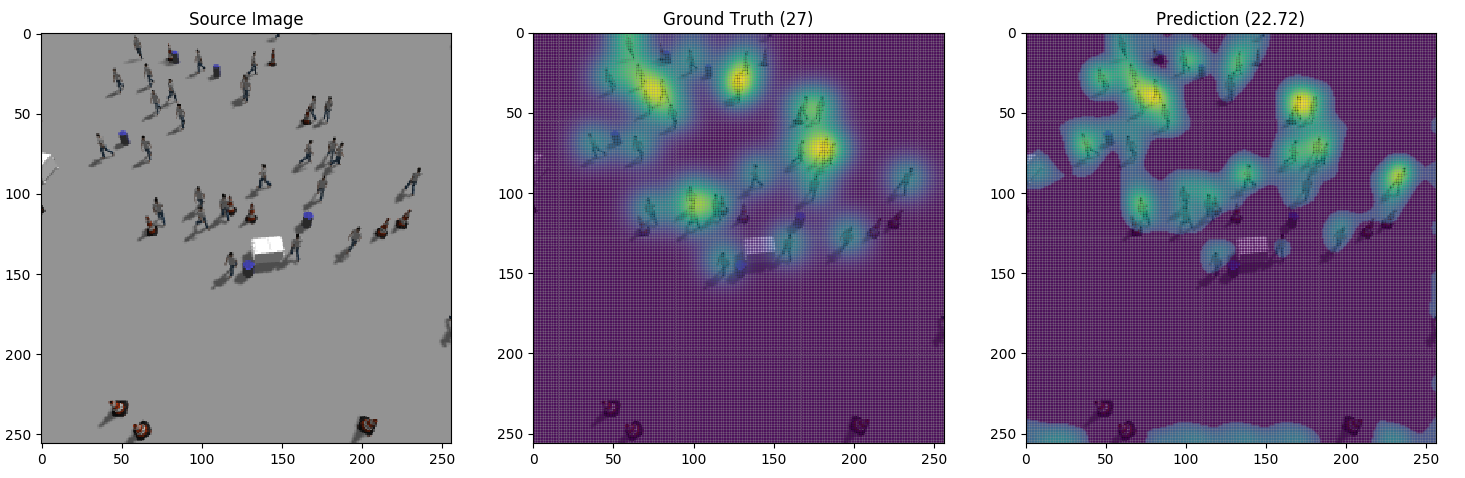
\includegraphics[width=0.9\linewidth]{img/example1.png}

  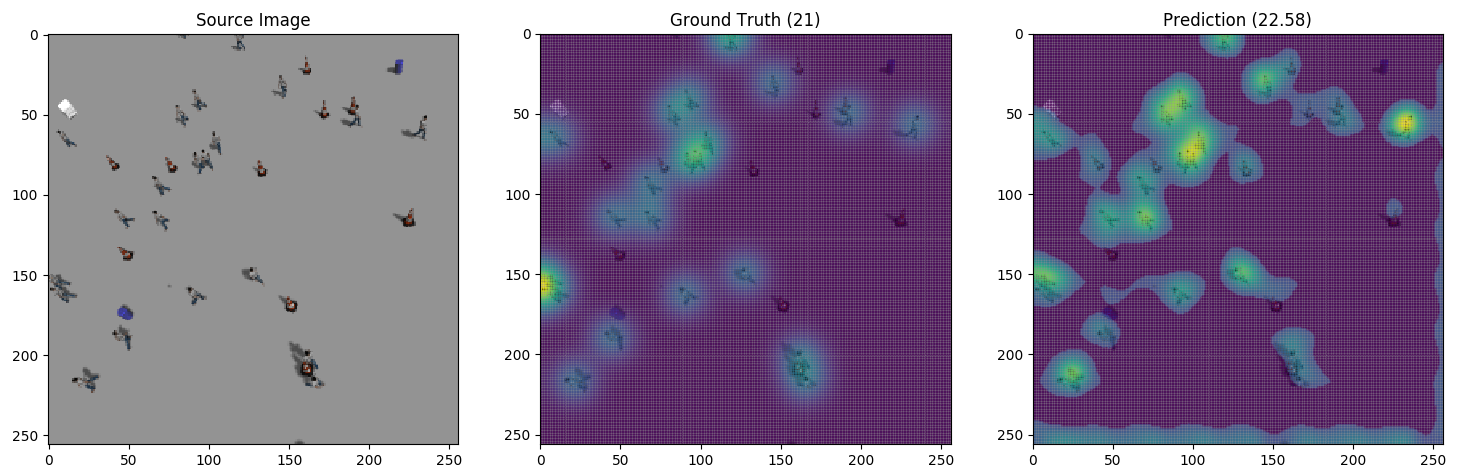
\includegraphics[width=0.9\linewidth]{img/example2.png}

  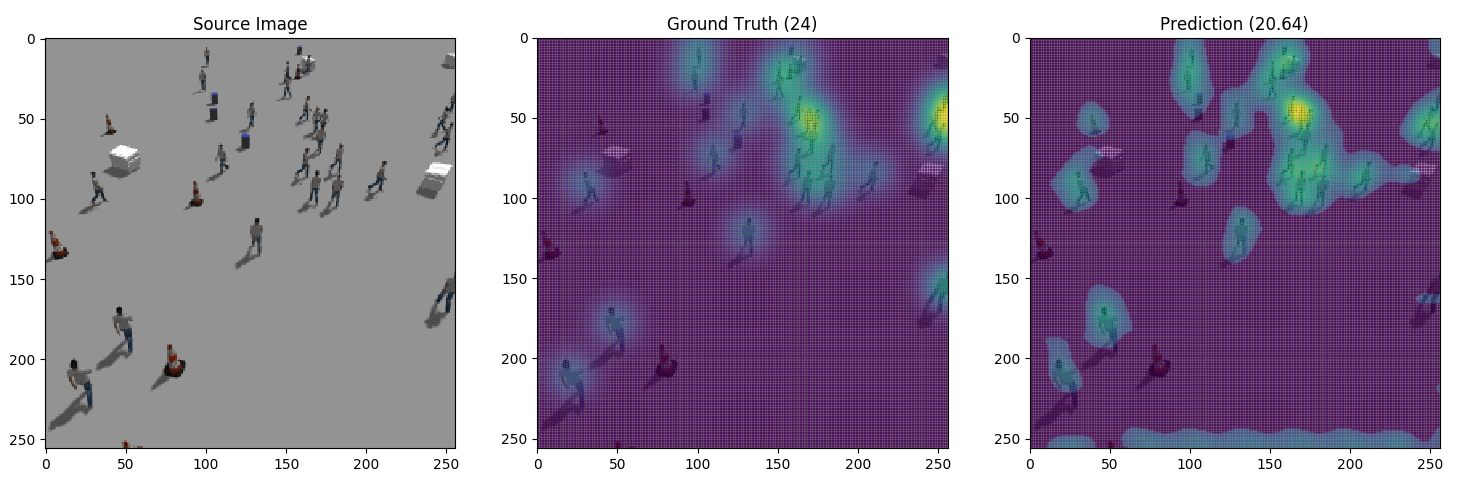
\includegraphics[width=0.9\linewidth]{img/example3.png}

  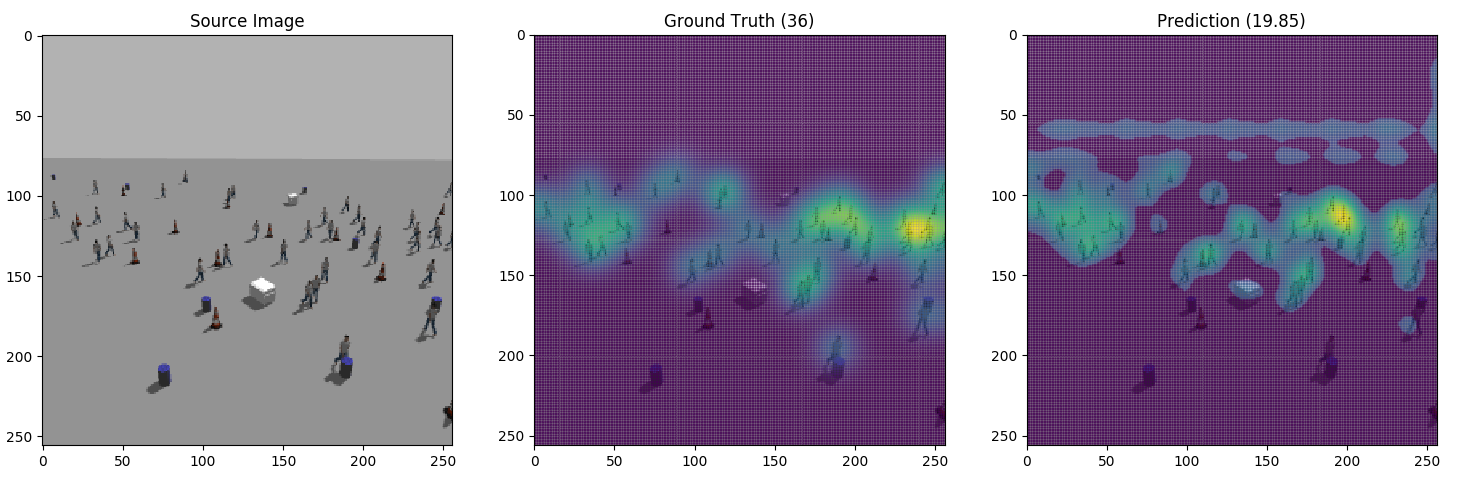
\includegraphics[width=0.9\linewidth]{img/example4.png}
  \end{center}
     \caption{Example output from the Counting CNN}
  \label{fig:ex1}
  \end{figure*}

%------------------------------------------------------------------------------
% SECTION 2: Gym Gazebo
%------------------------------------------------------------------------------

\section{Gym Gazebo}

  The OpenAI Gym~\cite{openaigym} is a popular reinforcement learning framework
  for simple tasks and games, which paces an agent through several training
  ``episodes'' in a custom ``environemnt''. Each episode provides positive or
  negative feedback to the training agent depending on the actions it takes
  based on its observations. Zamora et.al.\ of Erle Robotics extended this
  framework in \textit{Gym-Gazebo}~\cite{GymGazebo}, adding the ability to run
  this reinforcement learning cycle in Gazebo, and thus opening the framework
  to real-world robotics applications.

  Using this Gym-Gazebo, we can train a drone to accurately count the target
  population in an environment using reinforcement learning. The simulated
  drone used in this experiment is the Erle-Copter by Erle Robotics, a hobbyist
  quadrotor equipped with an autopilot and on-board camera. Erle Robotics
  provides a Erle-Copter simulation with the Gym-Gazebo distribution, which
  allows for us to conveniently hook our custom learning formulation into the
  pre-existing framework.

%------------------------------------------------------------------------------

\subsection{Learning Objective}
  
  Using the pre-trained Counting CNN to provide an estimate of the in-frame
  population count, we can train the drone to seek a pose which maximizes the
  estimated in-frame population. It is important to note that at this stage, it
  is assumed that the Counting CNN is a fixed structure in the observation
  pipeline, and not a trainable component. The Coutning CNN provides a noisy
  estimate of the in-frame population, which the agent can use to seek a higher
  reward. At this point, our objective is to learn the actions the drone should
  take to assume a pose which maximizes the observed count of the target
  population.

%------------------------------------------------------------------------------

\subsection{Reinforcement Learning Formulation}

  Reinforcement learning is an iterative process which gradually produces an
  intelligent model through reward-seeking behavior. Here we outline the
  primary formulation for learning how to maximize the observed target
  population class by a drone in an explorable environment.

  \begin{enumerate}
  \item \textbf{Environment}
    Training takes place in a static virtual Gazebo environment, which consists
    of a target class population (\textit{e.g.\ pedestrian models}) randomly
    distributed about the origin, along with randomly distributed accessory
    objects for noise.
  \item \textbf{Agent}
    The agent is a simulated Erle-Copter quadrotor drone, for which primary
    control is ``black-boxed'' through the on-board APM autopilot. The drone
    can takeoff, make aerial movements, and land using a simple command
    interface through ROS.
  \item \textbf{Observation Model}
    The primary observation for the learning context is the estimated target
    popultation count in the current frame. This is provided to the agent by
    passing the current frame through the pre-trained Counting CNN.
  \item \textbf{Action Model}
    The drone can take 8 actions to maximize its reward: moving either way in
    any of the 3 cardinal directions, plus rotating in either direction about
    its central axis.
  \item \textbf{Reward Model}
    The reward for each action is directly proportional to the population
    estimate. The more of the target population that the drone can accurately
    observe, the higher the reward.
  \end{enumerate}

%------------------------------------------------------------------------------

\section{Conclusions}

  The formulation described in this paper can be applied to any combination of
  target class, environment, and agent, depending on the problem at hand.
  Although this paper describes a single specific application (i.e.\ counting
  pedestrians with an aerial drone), it is a relatively simple exercise to
  adapt the pipeline to a different application, such as counting a particular
  species of coral using a submersible drone. The only requirements are a
  sufficiently detailed model of the target class, explorable environment, and
  agent control. 

%------------------------------------------------------------------------------
% Bibliography
%------------------------------------------------------------------------------

{\small
\bibliographystyle{ieee}
\bibliography{crowd_density}
}

\end{document}
